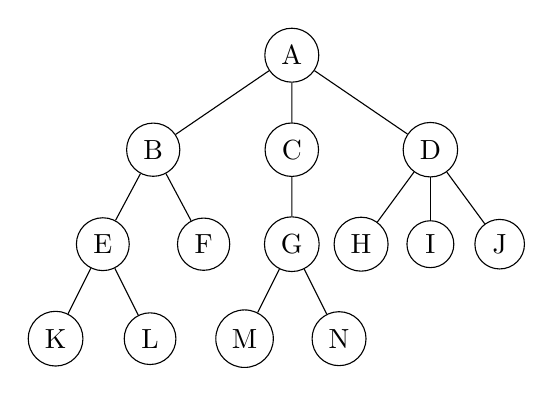
\begin{tikzpicture}[scale=0.8]

%% \tikzstyle{every node}=[ball color=red!70,circle,text=white]

\node[below right,circle,draw] at (2,0) {A}[sibling distance=2.2cm] 
  child { node[circle,draw]{B}[sibling distance=1.6cm]
	 child {node[circle,draw]{E}[sibling distance=1.5cm]
		child {node[circle,draw]{K}}
      child {node[circle,draw]{L}}
    }
	 child {node[circle,draw]{F}}      
  }
  child { node[circle,draw]{C}
    child {node[circle,draw]{G}[sibling distance=1.5cm]          
      child {node[circle,draw]{M}} 
      child {node[circle,draw]{N}}   
    }			
  }	
  child { node[circle,draw]{D}[sibling distance=1.1cm]
    child {node[circle,draw]{H}} 
    child {node[circle,draw]{I}}
    child {node[circle,draw]{J}}
  };  

%% \tikzstyle{every node}=[]
%\tikzstyle{information text}=[rounded corners,fill=blue!40!red!40,inner sep=1ex]
%\draw[xshift=6.2cm,yshift=0cm]
%node[below right,text width=4.6cm,style=information text]
%{
%该树的高度为4.
%};
% 
\end{tikzpicture}
